% =====================================================================
%  EL4201 Procesamiento Electrónico de Potencia - Proyecto 4
%  Etapa de potencia (Persona 2): puente H, modulación unipolar y
%  validación del modelo conmutado en PLECS
%  Compilar con pdflatex (dos pasadas). Probado también en Overleaf.
% =====================================================================
\documentclass[10pt,twocolumn,letterpaper]{article}

\usepackage[utf8]{inputenc}
\usepackage[T1]{fontenc}
\usepackage{lmodern}
\IfFileExists{spanish.ldf}{%
  \usepackage[spanish,es-tabla,es-nodecimaldot,es-noshorthands]{babel}%
}{%
  \usepackage[english]{babel}%
  \addto\captionsenglish{%
    \renewcommand{\figurename}{Figura}%
    \renewcommand{\tablename}{Tabla}%
    \renewcommand{\abstractname}{Resumen}%
    \renewcommand{\refname}{Referencias}%
    \renewcommand{\contentsname}{Contenido}}%
}
\usepackage[margin=1.8cm,columnsep=0.7cm]{geometry}
\usepackage{amsmath,amssymb}
\usepackage{graphicx}
\usepackage{booktabs}
\usepackage{array}
\usepackage{siunitx}
\sisetup{output-decimal-marker={,},group-separator={\,},per-mode=symbol}
\usepackage[americanvoltages,europeanresistors]{circuitikz}
\usetikzlibrary{calc}
\usepackage{caption}
\captionsetup{font=small,labelfont=bf}
\usepackage{stfloats}
\usepackage{xcolor}
\usepackage[hidelinks]{hyperref}

\newcommand{\prov}{\textsuperscript{\textdagger}}
\graphicspath{{../figuras/}}

\title{\textbf{Etapa de potencia del inversor monofásico:\\
puente H, modulación unipolar y modelo conmutado en PLECS}\\[4pt]
\large EL4201 Procesamiento Electrónico de Potencia --- Proyecto 4}
\author{[Nombre de la integrante] (Persona 2: puente H, accionamiento y protecciones)\\
Escuela de Ingeniería Electrónica, Tecnológico de Costa Rica}
\date{Avance del 4 de noviembre de 2026}

\begin{document}
\maketitle

\begin{abstract}
Se presenta el análisis de la etapa de potencia del inversor monofásico en puente H que alimenta la carga RL del proyecto. Se describen los estados de conmutación y los caminos de corriente, incluidos la conducción inversa por el canal de los MOSFET, la devolución de energía al bus y el efecto del tiempo muerto. Se formula la modulación PWM unipolar y se dimensionan, con parámetros provisionales, el margen de tensión, el rizado de corriente, los esfuerzos de los semiconductores y el capacitor de bus. Un modelo conmutado en PLECS, con el tiempo muerto implementado de forma explícita, confirma el patrón unipolar, un tiempo muerto de \SI{500}{\nano\second} y un rizado coincidente con la teoría. En lazo abierto, el error de amplitud de la fundamental es de $-5{,}6\,\%$ a \SI{1}{\ampere} y crece a $-26{,}9\,\%$ a \SI{0,2}{\ampere}; se demuestra que la causa es el error de tensión del tiempo muerto, que el regulador PR deberá compensar.
\end{abstract}

% ---------------------------------------------------------------------
\section{Alcance y parámetros de trabajo}
Este documento corresponde al paquete de la Persona~2 según la distribución del grupo: diseño del puente H, semiconductores, accionamiento, tiempo muerto y protecciones. Atiende la sección~5.3.2 del instructivo~\cite{instr} y aporta a 5.3.3 el modelo conmutado del puente y la relación entre modulación y tensión aplicada.

Mientras la carga y los componentes definitivos no estén seleccionados, se trabaja con los parámetros provisionales de la Tabla~\ref{tab:param}, marcados con \prov. Todos los cálculos se generan con scripts reproducibles (\texttt{calculos\_puente.py} y \texttt{analisis\_P2.py}) y se actualizarán con los valores medidos.

\begin{table}[!t]
\centering
\caption{Parámetros de trabajo. \prov: provisional.}
\label{tab:param}
\footnotesize
\begin{tabular}{@{}l l >{\raggedright\arraybackslash}p{3.0cm}@{}}
\toprule
Parámetro & Valor & Origen \\
\midrule
Tensión de bus $V_{dc}$ & \SI{24}{\volt}\prov & Máximo permitido (12--24 V) \\
Conmutación $f_{sw}$ & \SI{20}{\kilo\hertz}\prov & Se cierra en el diseño de pérdidas \\
Referencia $f_0$ & \SI{50}{\hertz} & Instructivo \\
$R_{ext}$ / $R_{dev}$ & \SI{8}{\ohm} / \SI{2}{\ohm}\prov & Persona 3 \\
$R_{tot}$ & \SI{10}{\ohm}\prov & $R_{ext}+R_{dev}$ \\
$L$ & \SI{20}{\milli\henry}\prov & Persona 3 \\
Tiempo muerto $t_{dt}$ & \SI{500}{\nano\second}\prov & Se recalcula con hojas de datos \\
$R_{DS(on)}$ & \SI{50}{\milli\ohm}\prov & MOSFET por elegir \\
$C_{bus}$ & \SI{470}{\micro\farad}, \SI{50}{\volt} & Sección~\ref{sec:bus} \\
\bottomrule
\end{tabular}
\end{table}

Se eligió $V_{dc}=\SI{24}{\volt}$ por dos razones: da el mayor margen de tensión para alcanzar \SI{1}{\ampere} pico con ambos valores de resistencia, y permite derivar la alimentación de \SI{12}{\volt} de los drivers del mismo bus mediante un regulador, de modo que basta una sola fuente.

% ---------------------------------------------------------------------
\section{Topología y estados de conmutación}
\subsection{Circuito}
El puente (Fig.~\ref{fig:puente}) está formado por dos piernas entre el bus positivo y la referencia. La pierna~A ($S_1$ arriba, $S_2$ abajo) define el nodo $a$, y la pierna~B ($S_3$, $S_4$) define el nodo $b$. La carga RL se conecta entre ambos nodos, de modo que la tensión aplicada es $v_{ab}=v_a-v_b$. Cada MOSFET incluye su diodo interno $D_1$--$D_4$. El capacitor $C_{bus}$ absorbe las corrientes pulsantes del puente y la energía que devuelve la carga.

\begin{figure}[!t]
\centering
\begin{circuitikz}[scale=0.76, transform shape, line width=0.6pt]
  \node[nmos, bodydiode, anchor=D] (S1) at (4.1,4) {};
  \node[nmos, bodydiode, anchor=D] (S2) at (S1.S) {};
  \node[nmos, bodydiode, anchor=D] (S3) at (8.9,4) {};
  \node[nmos, bodydiode, anchor=D] (S4) at (S3.S) {};
  \coordinate (top0) at (0,4);
  \coordinate (gnd0) at (top0 |- S2.S);
  \coordinate (cb) at (1.5,4);
  \draw (top0) to[V, l_=$V_{dc}$] (gnd0);
  \draw (top0) -- (S3.D);
  \draw (cb) to[C, l=$C_{bus}$, *-*] (cb |- gnd0);
  \draw (gnd0) -- (S4.S);
  \draw (S1.S) to[short, *-] ++(0.5,0) to[R, l=$R$] ++(1.7,0)
        to[L, l=$L$] ++(1.7,0) -- (S3.S) node[circ]{};
  \node[left=2pt] at (S1.G) {$S_1$};
  \node[left=2pt] at (S2.G) {$S_2$};
  \node[left=2pt] at (S3.G) {$S_3$};
  \node[left=2pt] at (S4.G) {$S_4$};
  \node[above left] at (S1.S) {$a$};
  \node[below left] at (S3.S) {$b$};
  \draw (S2.S) node[ground]{};
  \node[above] at (6,4) {bus $+$};
  \draw[->, thick, red!70!black] ($(S1.S)+(0.8,-0.4)$) -- ++(1.1,0)
        node[midway, below, font=\small] {$i>0$};
\end{circuitikz}
\caption{Inversor monofásico en puente H con la carga RL entre los nodos $a$ y $b$. El sentido positivo de la corriente es de $a$ hacia $b$.}
\label{fig:puente}
\end{figure}

\subsection{Estados permitidos}
En cada pierna los dos MOSFET operan de forma complementaria; encender ambos cortocircuita el bus (\emph{shoot-through}). Con esta restricción existen los cuatro estados de la Tabla~\ref{tab:estados}.

\begin{table}[!t]
\centering
\caption{Estados de conmutación (sin tiempo muerto).}
\label{tab:estados}
\small
\begin{tabular}{@{}lcccc@{}}
\toprule
Estado & Encendidos & $v_a$ & $v_b$ & $v_{ab}$ \\
\midrule
Positivo & $S_1$, $S_4$ & $V_{dc}$ & 0 & $+V_{dc}$ \\
Negativo & $S_3$, $S_2$ & 0 & $V_{dc}$ & $-V_{dc}$ \\
Cero superior & $S_1$, $S_3$ & $V_{dc}$ & $V_{dc}$ & 0 \\
Cero inferior & $S_2$, $S_4$ & 0 & 0 & 0 \\
\midrule
Prohibido & $S_1{+}S_2$ o $S_3{+}S_4$ & \multicolumn{3}{c}{cortocircuito del bus} \\
\bottomrule
\end{tabular}
\end{table}

\subsection{Caminos de corriente}
La Tabla~\ref{tab:caminos} resume, para cada estado y signo de la corriente, qué dispositivos conducen y hacia dónde fluye la energía. Se destacan tres fenómenos que condicionan el diseño:

\textbf{Conducción inversa por el canal.} Un MOSFET encendido conduce en ambos sentidos. Por ejemplo, en el estado positivo con $i<0$ la corriente circula de fuente a drenador por los canales de $S_4$ y $S_1$, no por los diodos. Los diodos solo conducen cuando los dos transistores de una pierna están apagados, es decir, durante el tiempo muerto.

\textbf{Devolución de energía al bus.} Por el carácter inductivo de la carga, la corriente se atrasa respecto de la tensión un ángulo $\varphi=\arctan(\omega L/R)$. Durante parte de cada semiciclo, $v_{ab}$ e $i$ tienen signos opuestos y la carga devuelve energía al bus. Una fuente de laboratorio no absorbe corriente, de modo que esa energía la recibe $C_{bus}$ (Sección~\ref{sec:bus}).

\textbf{Tensión durante el tiempo muerto.} Con ambos MOSFET de una pierna apagados, la tensión del nodo la fija el diodo que conduce, y este depende del signo de la corriente: en la pierna~A, con $i>0$ conduce $D_2$ ($v_a\approx-V_F$), y con $i<0$ conduce $D_1$ ($v_a\approx V_{dc}$). El resultado es un error de tensión que no controla el modulador (Sección~\ref{sec:dt}).

\begin{table}[!t]
\centering
\caption{Dispositivos en conducción y flujo de energía (inv.: conducción inversa por el canal).}
\label{tab:caminos}
\footnotesize
\setlength{\tabcolsep}{2.5pt}
\begin{tabular}{@{}lll@{}}
\toprule
Estado & $i>0$ ($a\to b$) & $i<0$ ($b\to a$) \\
\midrule
$+V_{dc}$ & $S_1$, $S_4$: entrega & $S_4$, $S_1$ (inv.): devuelve \\
$-V_{dc}$ & $S_2$, $S_3$ (inv.): devuelve & $S_3$, $S_2$: entrega \\
Cero sup. & $S_3$ (inv.), $S_1$: recircula & $S_1$ (inv.), $S_3$: recircula \\
Cero inf. & $S_4$, $S_2$ (inv.): recircula & $S_2$, $S_4$ (inv.): recircula \\
$t_{dt}$ pierna A & $D_2$: $v_a\approx 0$ & $D_1$: $v_a\approx V_{dc}$ \\
\bottomrule
\end{tabular}
\end{table}

% ---------------------------------------------------------------------
\section{Modulación PWM unipolar}
En PWM unipolar~\cite{mohan,holmes} las dos piernas se comparan con la misma portadora triangular $c(t)\in[-1,1]$: la pierna~A con el índice de modulación $+m$ y la pierna~B con $-m$. El transistor superior de cada pierna se enciende cuando su moduladora supera a la portadora (Fig.~\ref{fig:pwm}). Los ciclos de trabajo resultan
\begin{equation}
d_A=\frac{1+m}{2}, \qquad d_B=\frac{1-m}{2},
\end{equation}
y el promedio de la tensión en la carga, sobre un período de conmutación, es
\begin{equation}
\bar v_{ab}=(d_A-d_B)\,V_{dc}=m\,V_{dc}, \qquad -1\le m\le 1 .
\label{eq:vprom}
\end{equation}
La ecuación~\eqref{eq:vprom} es la ganancia del modulador que la Persona~1 incorpora a la planta: la salida del PR, una tensión, se divide entre $V_{dc}$ para obtener $m$.

Con $m>0$, $v_{ab}$ alterna entre $+V_{dc}$ y 0, usando ambos estados cero. Con $m<0$ alterna entre $-V_{dc}$ y 0. Cada transistor conmuta a $f_{sw}$, pero $v_{ab}$ presenta dos pulsos por período de portadora, de modo que su componente de conmutación predominante está en $2f_{sw}$. Esta es la distinción que exige el instructivo.

\begin{figure}[!t]
\centering
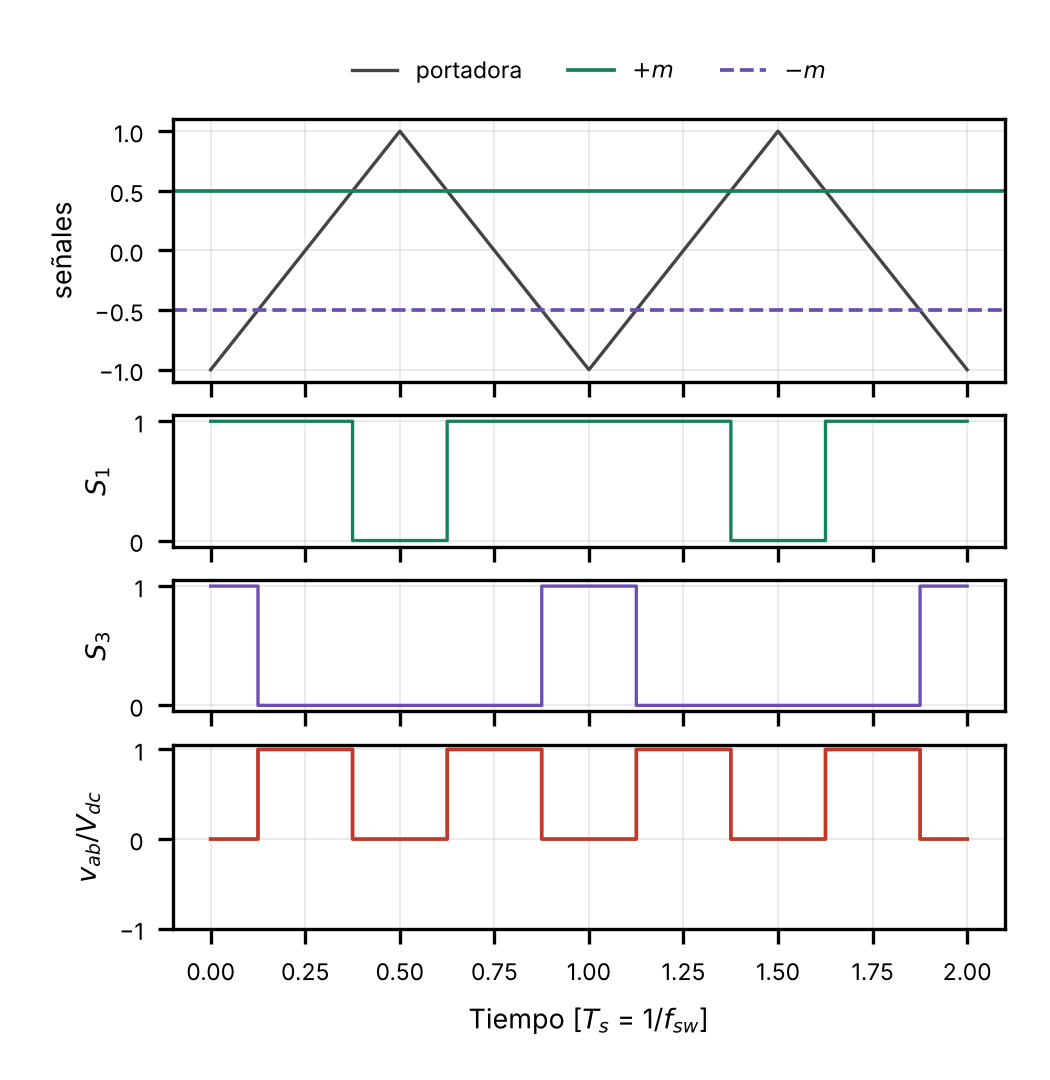
\includegraphics[width=\columnwidth]{pwm_unipolar_ideal.png}
\caption{PWM unipolar ideal con $m=0{,}5$: comparación de $\pm m$ con la portadora, compuertas superiores y tensión normalizada en la carga, con dos pulsos por período $T_s$.}
\label{fig:pwm}
\end{figure}

Como el período de conmutación es mucho menor que la constante de tiempo $L/R_{tot}$ (\SI{2}{\milli\second}), la corriente varía linealmente dentro de cada pulso y el rizado pico a pico de la corriente en PWM unipolar es~\cite{mohan,erickson}
\begin{equation}
\Delta i_{pp}=\frac{V_{dc}\,|m|\,(1-|m|)}{2\,L\,f_{sw}}, \qquad
\Delta i_{pp,\max}=\frac{V_{dc}}{8\,L\,f_{sw}},
\label{eq:rizado}
\end{equation}
con el máximo en $|m|=0{,}5$.

% ---------------------------------------------------------------------
\section{Dimensionamiento preliminar}
\subsection{Margen de tensión y rizado}
El índice necesario para cada punto de operación es $m_a=I_{pk}|Z|/V_{dc}$, con $|Z|=\sqrt{R_{tot}^2+(\omega_0 L)^2}$. Se exige $m_a\le 0{,}9$ para reservar margen de acción al regulador. La Tabla~\ref{tab:margen} muestra que todos los puntos, incluido el cambio de $R_{ext}$ en $+25\,\%$, quedan holgados ($m_a\le 0{,}56$), y que el rizado máximo (\SI{7,5}{\milli\ampere}) es más de 25 veces menor que el límite de \SI{0,20}{\ampere}. Esto indica que $L$ o $f_{sw}$ podrían reducirse si las pérdidas lo justifican.

\begin{table*}[!t]
\centering
\caption{Margen de tensión y rizado máximo en los puntos de operación ($V_{dc}=\SI{24}{\volt}$, $f_{sw}=\SI{20}{\kilo\hertz}$, $L=\SI{20}{\milli\henry}$).}
\label{tab:margen}
\small
\begin{tabular}{@{}cccccccc@{}}
\toprule
$R_{tot}$ [\si{\ohm}] & $I_{pk}$ [A] & $|Z|$ [\si{\ohm}] & $\varphi$ [$^\circ$] & $V_{pk}$ requerida [V] & $m_a$ & $m_a\le 0{,}9$ & $\Delta i_{pp,\max}$ [mA] \\
\midrule
10 & 0,2 & 11,81 & 32,1 & 2,36 & 0,098 & Sí & 2,66 \\
10 & 0,5 & 11,81 & 32,1 & 5,91 & 0,246 & Sí & 5,57 \\
10 & 1,0 & 11,81 & 32,1 & 11,81 & 0,492 & Sí & 7,50 \\
12 ($R_{ext}+25\,\%$) & 0,5 & 13,55 & 27,6 & 6,77 & 0,282 & Sí & 6,08 \\
12 ($R_{ext}+25\,\%$) & 1,0 & 13,55 & 27,6 & 13,55 & 0,564 & Sí & 7,50 \\
\bottomrule
\end{tabular}
\end{table*}

\subsection{Esfuerzos en los semiconductores}
Cada MOSFET bloquea $V_{dc}$ más las sobretensiones de conmutación por inductancias parásitas. Con un factor de seguridad de 2,5 se requiere $V_{DSS}\ge\SI{60}{\volt}$. Las corrientes son bajas para cualquier MOSFET de potencia (Tabla~\ref{tab:esfuerzos}). La corriente pico de diseño de \SI{2}{\ampere} cubre los transitorios de consigna y de carga, y se adopta como umbral provisional de la protección de sobrecorriente.

\begin{table}[!t]
\centering
\caption{Esfuerzos eléctricos por MOSFET a \SI{1}{\ampere} pico.}
\label{tab:esfuerzos}
\footnotesize
\begin{tabular}{@{}lll@{}}
\toprule
Magnitud & Valor & Criterio \\
\midrule
Bloqueo $V_{DS}$ & \SI{24}{\volt} & $V_{DSS}\ge\SI{60}{\volt}$ \\
$I_{D}$ pico & \SI{1,004}{\ampere} & $I_{pk}+\Delta i_{pp}/2$ \\
$I_{D}$ pico de diseño & \SI{2,0}{\ampere} & Transitorios, protección \\
$I_{rms}$ de la carga & \SI{0,707}{\ampere} & $I_{pk}/\sqrt2$ \\
$I_{rms}$ por MOSFET & \SIrange{0,50}{0,71}{\ampere} & Típico a cota \\
\bottomrule
\end{tabular}
\end{table}

\subsection{Bus DC y capacitor}\label{sec:bus}
La potencia en la carga a \SI{1}{\ampere} pico es $R_{tot}I_{pk}^2/2=\SI{5}{\watt}$, de los cuales \SI{4}{\watt} se disipan en $R_{ext}$; con resistencias de \SI{5}{\watt} el margen es insuficiente y se recomienda una de \SI{10}{\watt} o varias en paralelo. La corriente media del bus es de \SI{0,21}{\ampere}.

La energía devuelta en cada intervalo regenerativo se obtiene integrando la potencia instantánea negativa $p=v\,i$, con $v=R_{tot}\,i+L\,\mathrm{d}i/\mathrm{d}t$:
\begin{equation}
E_{reg}=\int_{p<0}|v\,i|\,\mathrm{d}t=\SI{1,07}{\milli\joule}\quad(\SI{1}{\ampere}\text{ pico}).
\end{equation}
Si la fuente no absorbe corriente, toda esa energía la recibe el capacitor, y la tensión del bus sube aproximadamente $\Delta V\approx E_{reg}/(C_{bus}V_{dc})$: \SI{203}{\milli\volt}, \SI{95}{\milli\volt} y \SI{45}{\milli\volt} para \SIlist{220;470;1000}{\micro\farad}. Se selecciona $C_{bus}=\SI{470}{\micro\farad}$, \SI{50}{\volt} ($\ge 1{,}5\,V_{dc}$), electrolítico, complementado con un cerámico de \SIrange{0,1}{1}{\micro\farad} junto a cada pierna para las corrientes de alta frecuencia.

% ---------------------------------------------------------------------
\section{Modelo conmutado en PLECS}
El modelo en PLECS~\cite{plecs} (Fig.~\ref{fig:plecs}) representa la fuente de laboratorio como una fuente ideal con resistencia interna y un diodo en serie que impide la circulación de corriente inversa. Así, la energía regenerada solo puede almacenarse en $C_{bus}$, como ocurre en el montaje real. Los interruptores son MOSFET con su diodo en antiparalelo. La corriente de carga y las tensiones $v_{ab}$ y $V_{bus}$ se registran con medidores. Todos los valores se toman de un único bloque de inicialización (\texttt{parametros\_puente.m}), cuyos nombres de variable son comunes a todo el grupo.

\begin{figure*}[!t]
\centering
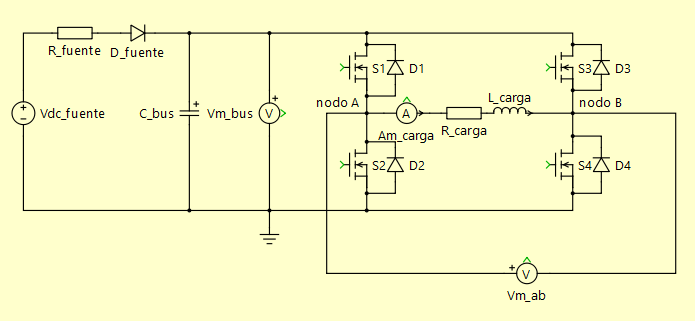
\includegraphics[width=0.72\textwidth]{plecs_esquema_potencia.png}
\caption{Circuito de potencia en PLECS: fuente con $R_{fuente}$ y $D_{fuente}$, $C_{bus}$, piernas $S_1$--$S_4$ con diodos $D_1$--$D_4$, carga RL y medidores.}
\label{fig:plecs}
\end{figure*}

El modulador reproduce la comparación unipolar con bloques elementales, para que su lógica coincida con la del periférico PWM que implementa Taller. El tiempo muerto se obtiene retrasando solo el flanco de subida de cada compuerta:
\begin{equation}
g_1 = x_A \wedge x_A(t-t_{dt}), \qquad g_2=\bar x_A\wedge\bar x_A(t-t_{dt}),
\end{equation}
donde $x_A$ es la salida del comparador de la pierna~A. El retardo se implementa con bloques \emph{Pulse Delay}, adecuados para señales discretas. La Tabla~\ref{tab:bloques} lista los bloques de control y sus parámetros.

\begin{table}[!t]
\centering
\caption{Bloques del modulador en PLECS.}
\label{tab:bloques}
\small
\setlength{\tabcolsep}{3pt}
\begin{tabular}{@{}lll@{}}
\toprule
Bloque & Nombre & Parámetros \\
\midrule
Sine Wave Gen. & \texttt{m\_ref} & $m_a$, $2\pi f_0$ rad/s \\
Triangular Wave Gen. & \texttt{portadora} & $[-1,1]$, $f_{sw}$, 0,5 \\
Gain & \texttt{inv\_m} & $-1$ \\
Relational Op. ($>$) & \texttt{comp\_A}, \texttt{comp\_B} & --- \\
Logical Op. (NOT) & \texttt{NOT\_A}, \texttt{NOT\_B} & --- \\
Pulse Delay & \texttt{dt\_S1}--\texttt{dt\_S4} & $t_{dt}$ \\
Logical Op. (AND) & \texttt{AND\_S1}--\texttt{AND\_S4} & 2 entradas \\
\bottomrule
\end{tabular}
\end{table}

% ---------------------------------------------------------------------
\section{Resultados de simulación}
\subsection{P1: estados con índice constante}
Con $m=0{,}5$ constante (Fig.~\ref{fig:p1}), $v_{ab}$ alterna entre $+V_{dc}$ y 0 a \SI{40}{\kilo\hertz} ($2f_{sw}$), sin pasar por $-V_{dc}$, con promedio $mV_{dc}=\SI{12}{\volt}$. La corriente crece como la respuesta al escalón de la carga RL: la teoría predice $i(\SI{1}{\milli\second})=1{,}2\,(1-e^{-0{,}5})=\SI{0,472}{\ampere}$, y la simulación da \SI{0,45}{\ampere}. La diferencia corresponde a las pérdidas en $R_{DS(on)}$, $R_{fuente}$ y al tiempo muerto.

\begin{figure*}[!t]
\centering
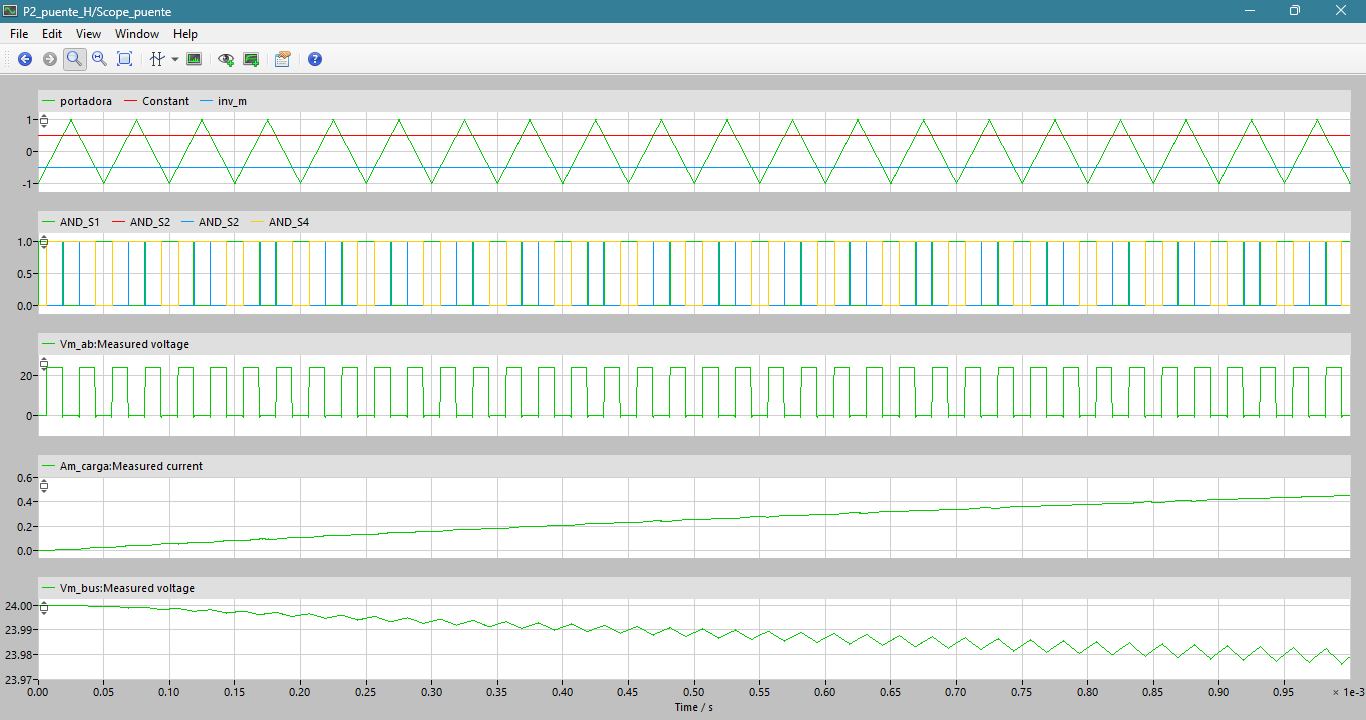
\includegraphics[width=0.85\textwidth]{P1_estados_m05.png}
\caption{Prueba P1 ($m=0{,}5$ constante): portadora y $\pm m$, compuertas, $v_{ab}$, corriente de carga y tensión de bus durante \SI{1}{\milli\second}.}
\label{fig:p1}
\end{figure*}

\subsection{P3: tiempo muerto}
La Fig.~\ref{fig:p3} muestra las compuertas de la pierna~A. Con la portadora cruzando $m=0{,}5$ en \SI{18,75}{\micro\second}, $g_1$ se apaga en ese instante y $g_2$ se enciende en \SI{19,25}{\micro\second}. En el flanco opuesto, $g_2$ se apaga en \SI{31,25}{\micro\second} y $g_1$ se enciende en \SI{31,75}{\micro\second}. En ambos sentidos el intervalo con las dos compuertas apagadas es de \SI{500}{\nano\second}, y en ningún instante coinciden encendidas. El tiempo muerto se aplica también al arranque.

\begin{figure}[!t]
\centering
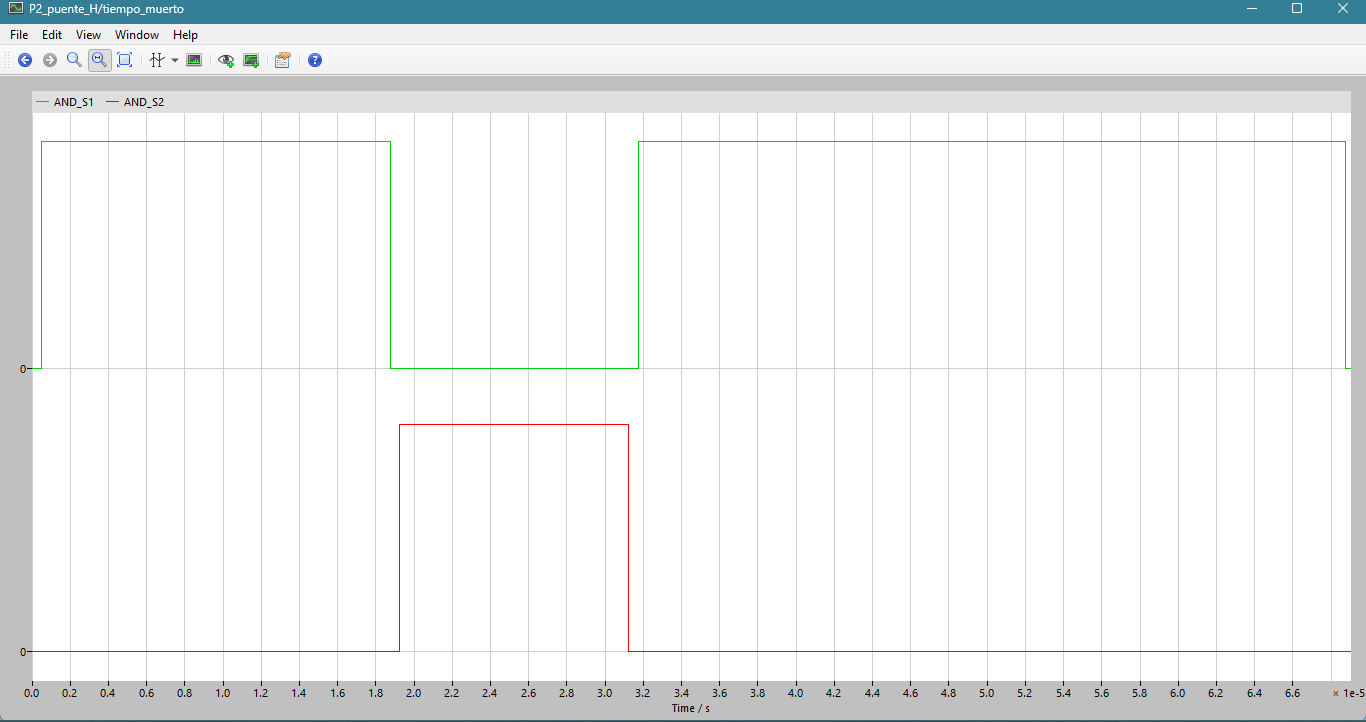
\includegraphics[width=\columnwidth]{P3_tiempo_muerto_A.png}
\caption{Compuertas $g_1$ (arriba) y $g_2$ (abajo) de la pierna~A: tiempo muerto de \SI{500}{\nano\second} en ambos flancos.}
\label{fig:p3}
\end{figure}

\subsection{P2: referencia senoidal en lazo abierto}
Se aplicó $m(t)=m_a\sin(\omega_0 t)$ con $m_a$ calculado para cada corriente (Tabla~\ref{tab:margen}), sin regulador. Los datos exportados de PLECS se procesaron con el método del instructivo (sección~5.3.5):
\begin{itemize}\setlength\itemsep{1pt}
\item Ventana de los últimos cinco períodos completos de \SI{50}{\hertz} (\SIrange{0,10}{0,20}{\second}), en régimen periódico, remuestreada uniformemente a \SI{0,5}{\micro\second}.
\item Fundamental de corriente y tensión por proyección a \SI{50}{\hertz}. El desfase se mide entre las fundamentales de $m$ y de $i$.
\item Componente de baja frecuencia: armónicos hasta \SI{2}{\kilo\hertz}. El rizado de conmutación es la diferencia entre la corriente y esa componente, medido pico a pico en ventanas locales de \SI{1}{\milli\second}; se reporta el máximo.
\end{itemize}

\begin{table*}[!t]
\centering
\caption{Resultados de la prueba P2 (lazo abierto) sobre cinco períodos en régimen.}
\label{tab:p2}
\small
\begin{tabular}{@{}ccccccccc@{}}
\toprule
$I_{ref}$ [A] & $m_a$ & $I_1$ [A] & Error [\%] & Desfase [$^\circ$] & $V_1$ [V] & $m_aV_{dc}$ [V] & $\Delta i_{pp}$ sim. [mA] & $\Delta i_{pp}$ teór. [mA] \\
\midrule
0,2 & 0,098 & 0,146 & $-26{,}9$ & 25,5 & 1,805 & 2,362 & 2,75 & 2,66 \\
0,5 & 0,246 & 0,447 & $-10{,}6$ & 28,8 & 5,320 & 5,905 & 5,23 & 5,57 \\
1,0 & 0,492 & 0,944 & $-5{,}6$ & 30,2 & 11,196 & 11,810 & 7,50 & 7,50 \\
\bottomrule
\end{tabular}
\end{table*}

La Tabla~\ref{tab:p2} resume los resultados. El rizado simulado coincide con la ecuación~\eqref{eq:rizado} con diferencias menores que \SI{0,4}{\milli\ampere}, lo que valida la relación entre $f_{sw}$, $L$ y rizado en PWM unipolar (Fig.~\ref{fig:rizado}). En cambio, la amplitud de la fundamental queda por debajo de la referencia, y el error relativo crece al bajar la corriente.

\begin{figure}[!t]
\centering
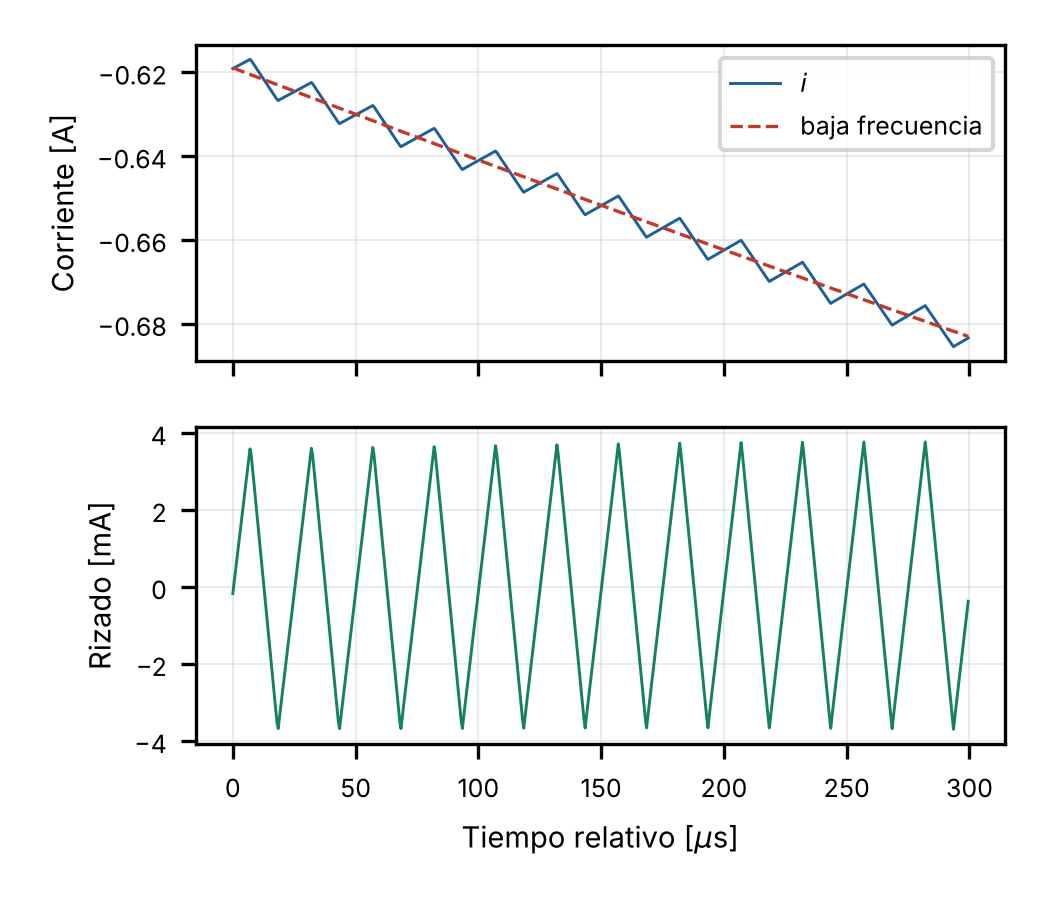
\includegraphics[width=\columnwidth]{P2_rizado_1p0A.png}
\caption{Separación del rizado de conmutación a \SI{1}{\ampere} pico: corriente y componente de baja frecuencia (arriba) y rizado resultante, \SI{7,5}{\milli\ampere} pico a pico (abajo).}
\label{fig:rizado}
\end{figure}

\subsection{Efecto del tiempo muerto}\label{sec:dt}
Según el análisis clásico del tiempo muerto~\cite{holmes,mohan}, en cada período de conmutación y en cada pierna este sustituye durante $t_{dt}$ la tensión deseada por la que fija el diodo. Esto produce un error medio de $V_{dc}t_{dt}f_{sw}$ por pierna, con signo opuesto al de la corriente. En el puente completo el error es una onda cuadrada en fase con $i$, de amplitud $2V_{dc}t_{dt}f_{sw}=\SI{0,48}{\volt}$, cuya fundamental vale
\begin{equation}
\Delta V_1=\frac{4}{\pi}\,2V_{dc}t_{dt}f_{sw}=\SI{0,611}{\volt}.
\end{equation}
La pérdida simulada de fundamental, $m_aV_{dc}-V_1$, es de \SIlist{0,557;0,585;0,614}{\volt} para \SIlist{0,2;0,5;1,0}{\ampere}. Es prácticamente constante y coincide con la predicción. Como es un error de tensión fijo, pesa \SI{24}{\percent} de la tensión necesaria a \SI{0,2}{\ampere} y solo \SI{5}{\percent} a \SI{1}{\ampere}, lo que explica la tendencia del error.

Al estar en fase con la corriente, el error actúa como una resistencia equivalente $R_{eq}=\Delta V_1/I_1$, de \SIlist{3,81;1,31;0,65}{\ohm}. Con ella, el desfase predicho $\arctan[\omega_0L/(R_{tot}+R_{eq})]$ resulta \SIlist{24,5;29,1;30,5}{\degree}, frente a \SIlist{25,5;28,8;30,2}{\degree} simulados. Esto explica la reducción del desfase respecto de los \SI{32,1}{\degree} nominales. El mismo fenómeno aplana la corriente cerca de sus cruces por cero (Fig.~\ref{fig:i02}).

\begin{figure}[!t]
\centering
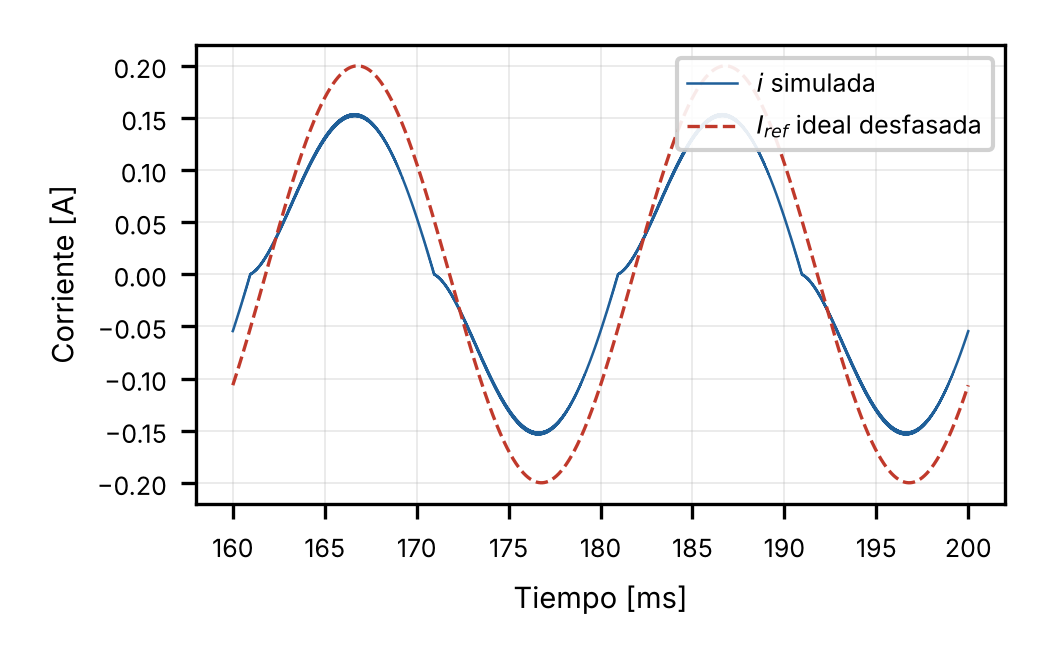
\includegraphics[width=\columnwidth]{P2_corriente_0p2A.png}
\caption{Corriente a \SI{0,2}{\ampere} pico en lazo abierto frente a la referencia ideal desfasada: amplitud reducida y distorsión en los cruces por cero por el tiempo muerto.}
\label{fig:i02}
\end{figure}

Dos consecuencias para el diseño: (i) en lazo abierto no se cumple el criterio del \SI{10}{\percent} a \SI{0,2}{\ampere} ni, por poco, a \SI{0,5}{\ampere}; la corrección corresponde al regulador PR, cuya ganancia resonante elimina el error en la fundamental, y la Persona~1 debe considerar esta perturbación al sintonizarlo; (ii) el error es proporcional a $t_{dt}f_{sw}$, por lo que el tiempo muerto debe ser el mínimo seguro según las hojas de datos y no un valor holgado.

\subsection{P4: tensión de bus}
La Fig.~\ref{fig:bus} muestra $v_{ab}$ y $V_{bus}$ a \SI{1}{\ampere} pico durante un ciclo. Los pulsos cambian de polaridad en cada semiciclo, como corresponde al patrón unipolar. El bus sube hasta \SI{24,087}{\volt} en los dos intervalos regenerativos de cada ciclo, entre el cruce por cero de la tensión y el de la corriente. Es una elevación de \SI{87}{\milli\volt}, frente a \SI{95}{\milli\volt} estimados en la Sección~\ref{sec:bus}, lo que confirma el dimensionamiento de $C_{bus}$. En los intervalos de entrega el bus baja hasta \SI{23,953}{\volt} por la caída en $R_{fuente}$.

\begin{figure}[!t]
\centering
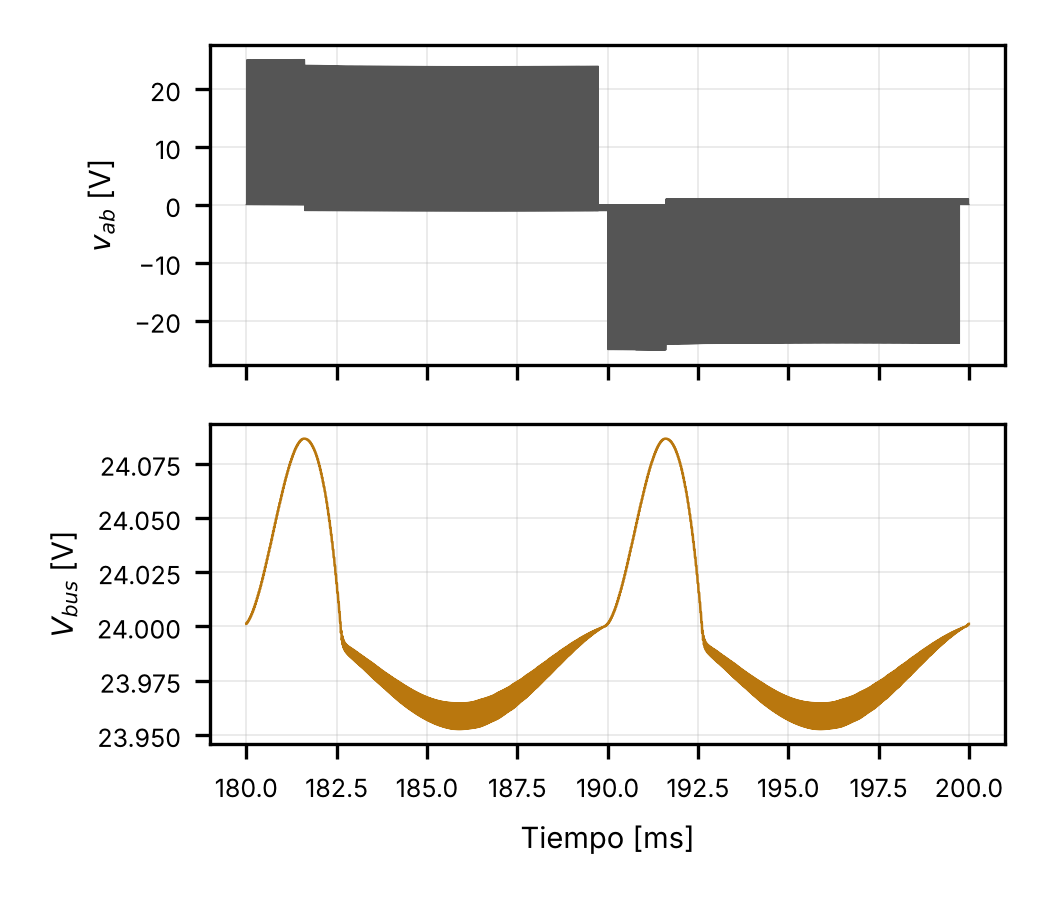
\includegraphics[width=\columnwidth]{P2_vab_bus_1p0A.png}
\caption{Tensión en la carga y tensión de bus a \SI{1}{\ampere} pico: cambio de polaridad unipolar y elevación del bus por la energía regenerada.}
\label{fig:bus}
\end{figure}

% ---------------------------------------------------------------------
\section{Conclusiones parciales y trabajo pendiente}
\begin{itemize}\setlength\itemsep{1pt}
\item El modelo conmutado reproduce el patrón unipolar, la componente de conmutación a $2f_{sw}$, el tiempo muerto configurado y el rizado previsto. Es la base para el archivo integrado del grupo.
\item Con $V_{dc}=\SI{24}{\volt}$ todos los puntos de operación tienen margen ($m_a\le0{,}56$), y el rizado es muy inferior al límite.
\item El tiempo muerto introduce un error de tensión fundamental de unos \SI{0,6}{\volt}, dominante a baja corriente. Se comunica a la Persona~1 junto con $R_{eq}$ para el diseño del PR.
\item $C_{bus}=\SI{470}{\micro\farad}$ limita la elevación del bus por regeneración a menos de \SI{0,1}{\volt}.
\end{itemize}
Pendiente: selección de MOSFET y drivers con sus hojas de datos; cálculo del tiempo muerto mínimo; alimentación y referencias del accionamiento; pérdidas y cierre de $f_{sw}$; diseño de protecciones y desconexión; comprobación de compuertas con el bus desenergizado. Todos los valores marcados con \prov\ se actualizarán con los parámetros definitivos.

\begin{thebibliography}{9}\small
\bibitem{instr} J.~González-Gómez, Y.~Arias-Esquivel y R.~Coto Calderón, \emph{Proyecto~4: Control de corriente en un inversor monofásico mediante un regulador PR discreto sobre MicroBlaze~V}, Instructivo, EL3313/EL4201, TEC, II Semestre 2026.
\bibitem{mohan} N.~Mohan, T.~M.~Undeland y W.~P.~Robbins, \emph{Power Electronics: Converters, Applications, and Design}, 3.ª ed. Hoboken, NJ: Wiley, 2003.
\bibitem{holmes} D.~G.~Holmes y T.~A.~Lipo, \emph{Pulse Width Modulation for Power Converters: Principles and Practice}. Piscataway, NJ: IEEE Press/Wiley, 2003.
\bibitem{erickson} R.~W.~Erickson y D.~Maksimović, \emph{Fundamentals of Power Electronics}, 2.ª ed. Norwell, MA: Kluwer, 2001.
\bibitem{plecs} Plexim GmbH, \emph{PLECS User Manual}. Zúrich: Plexim.
\end{thebibliography}

\end{document}
